\chapter{Methodology}
\section{Baselines and Architecture}
\textbf{EfficientNet Baseline:} ImageNet\textendash pretrained EfficientNetB0 (optionally B3) with a light classification head: BN $\rightarrow$ Conv1x1 (192) $\rightarrow$ GAP $\rightarrow$ Dropout(0.4) $\rightarrow$ Dense(192, ReLU) $\rightarrow$ Dropout(0.4) $\rightarrow$ Softmax.

\textbf{EfficientNet + CBAM:} Same backbone and head, with a CBAM block applied on the convolutional feature map to apply channel and spatial attention.

% 1) Start with attention concept + base attention figure
\begin{figure}[t]
  \centering
  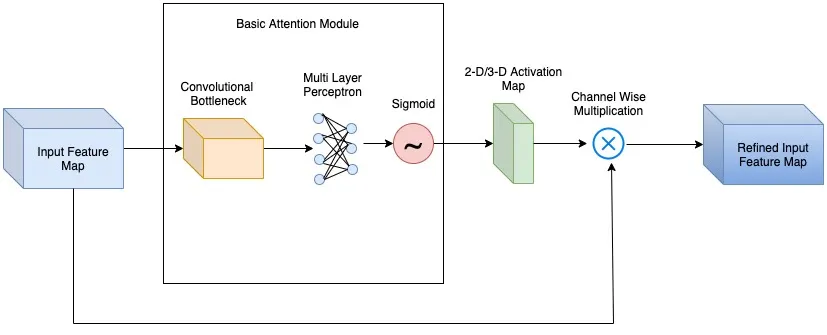
\includegraphics[width=0.9\textwidth]{../new_work/figures/about-cbam/base-attention-model.png}
  \caption{Base attention idea: an attention map refines intermediate feature maps to emphasize informative content and suppress background, improving downstream classification. Adapted for context from primers \cite{cbamMedium}.}
  \label{fig:base_attention}
\end{figure}

\subsection{CBAM Details}
CBAM introduces lightweight attention along two axes \cite{woo2018cbam,cbamMedium,cbamDO}:
\begin{itemize}
  \item \textbf{Channel attention (what):} statistics are pooled via both global average and max pooling and passed through a shared MLP to produce per\textendash channel weights in $(0,1)$ via $\sigma$. This emphasizes informative feature channels while suppressing less useful ones.
  \item \textbf{Spatial attention (where):} the feature map is aggregated across channels using average and max projections and filtered by a $7\times7$ convolution to produce a spatial mask highlighting salient regions.
  \item \textbf{Sequential composition:} channel attention is applied first, followed by spatial attention, i.e., $F' = M_s(M_c(F)\odot F)\odot F$. This ordering empirically outperforms the reverse or parallel setups.
  \item \textbf{Design contrasts to BAM:} unlike BAM that uses dilated convolutions to enlarge receptive fields, CBAM relies on a larger kernel ($7\times7$) with standard dilation and augments average pooling with max pooling, improving saliency capture \cite{cbamMedium}.
\end{itemize}

\begin{figure}[t]
  \centering
  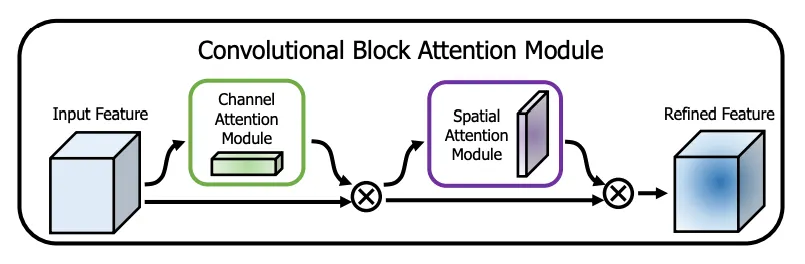
\includegraphics[width=0.95\textwidth]{../new_work/figures/about-cbam/cbam-architecture.png}
  \caption{CBAM module: sequential channel and spatial attention with shared MLP for channel pooling (Avg/Max) and a $7\times7$ conv for spatial pooling. See \cite{woo2018cbam,cbamMedium,cbamDO}.}
  \label{fig:cbam_module}
\end{figure}

% 3) Finally, our EfficientNet + CBAM integration
\begin{figure}[t]
  \centering
  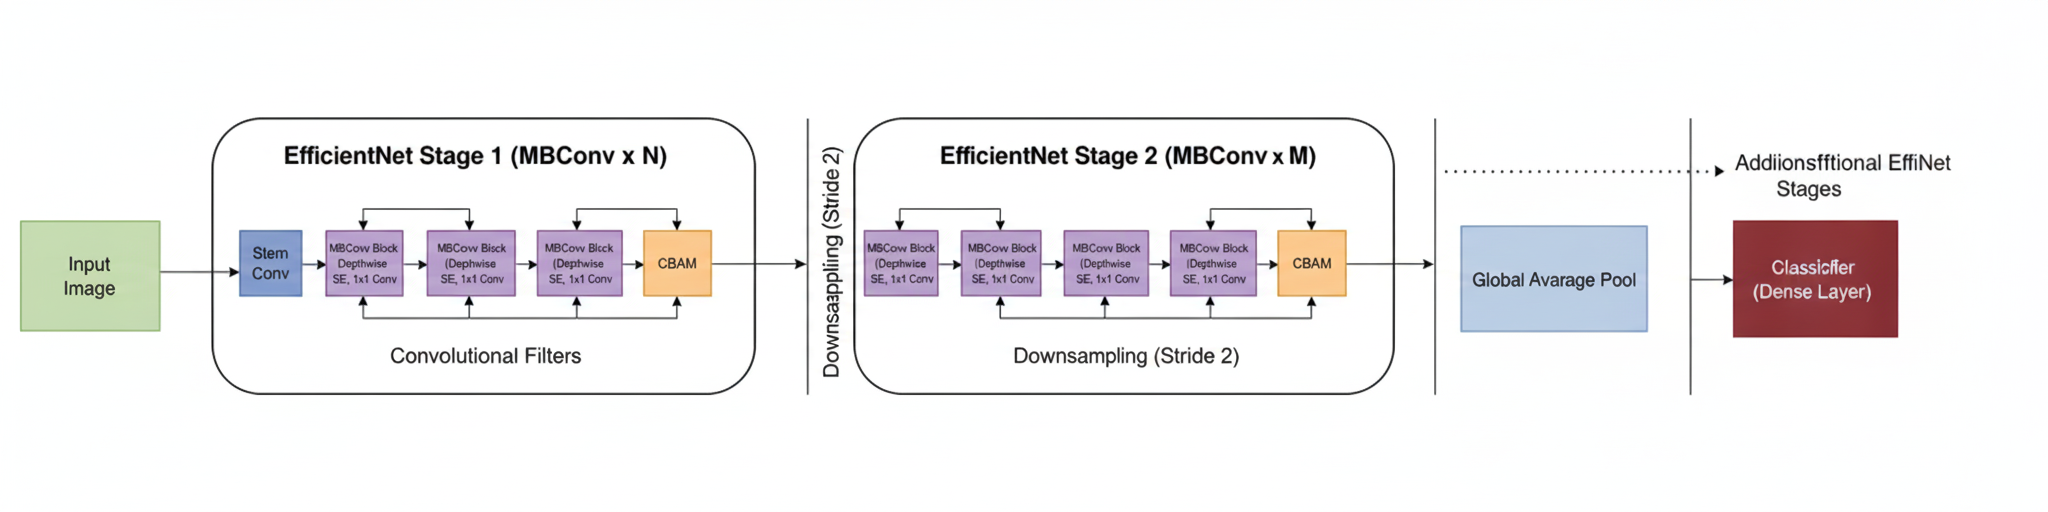
\includegraphics[width=0.9\textwidth]{../new_work/figures/about-cbam/EfficientNet-placement-with-CBAM-architecture.png}
  \caption{Our architecture: EfficientNet backbone with a CBAM attention block over feature maps, followed by a lightweight classification head.}
  \label{fig:cbam_arch}
\end{figure}

\section{Training}
Optimizer: Adam (lr $3\times10^{-4}$), batch size 16, warm\textendash up forward pass, callbacks: ModelCheckpoint (best val acc), ReduceLROnPlateau, EarlyStopping. Mixed precision is enabled for memory efficiency.

\paragraph{Loss and Metrics.} We optimize categorical cross\textendash entropy over 5 classes (G, C, A, H, M). We report accuracy; macro and weighted F1; ROC\textendash AUC (macro, one\textendash vs\textendash rest); and PR\textendash AUC (macro). Let $\hat{y}\_{i,c}$ be the predicted probability for class $c$; $y\_{i,c}\in\{0,1\}$. The loss is $\mathcal{L}= -\sum\_{i}\sum\_{c} y\_{i,c}\log(\hat{y}\_{i,c})$; macro F1 is the unweighted mean across classes.

\section{Evaluation}
We report accuracy, macro/weighted F1, ROC\textendash AUC (macro one\textendash vs\textendash rest), PR\textendash AUC (macro), and confusion matrices. Curves (training/validation for accuracy, loss, ROC\textendash AUC, PR\textendash AUC) and per\textendash class ROC/PR curves are exported.

\paragraph{CBAM Primer.} CBAM sequentially applies channel attention and spatial attention \cite{woo2018cbam}, reweighting feature channels (\emph{what}) and spatial locations (\emph{where}). We reference succinct primers \cite{cbamMedium,cbamDO} for intuition and module design.

\paragraph{Implementation Notes.} We integrate CBAM after the final EfficientNet convolutional block and before the classification head (Figure~\ref{fig:cbam_arch}). Channel attention uses a shared MLP with reduction ratio $r=16$; spatial attention uses a $7\times7$ convolution on concatenated average and max projections, following \cite{woo2018cbam,cbamDO}. We row\textendash normalize confusion matrices to percentages to reflect per\textendash class error structure.

